% Source printed pp. 302-307 / PDF pp. 310-315.
\section{\texorpdfstring{$\overline M_g$}{稳定曲线粗模空间}的几何一瞥}\label{src:6.10}
\begin{epigraph}
当 [Zariski] 说出``代数簇''时, 他的声音有一种共鸣, 清楚地表明他正凝视一个秘密花园. 我立即也想拥有这种能力\ldots\ 尤其是, 我迷上了这花园中的一种西番莲: Riemann 模空间.
\epigraphauthor{David Mumford~\cite[225 页]{AI97}}
\end{epigraph}
存在性, 不可约性和射影性 (定理~\hyperref[thm:A]{A}) 当然只是研究 $\overline M_g$ 的起点. 现在可以开始提出各种几何问题:
\begin{itemize}
\item 它的丰沛锥或有效锥是什么?
\item 它的 Kodaira 维数或典范模型是什么?
\item 粗模空间有什么奇点?
\item 它的奇异上同调, Chow 上同调或 Hodge 上同调是什么?
\item 对整数 $r,\allowbreak d$, 一般的亏格 $g$ 曲线是否具有一个 $g_d^r$?
\end{itemize}
注意, 甚至要讨论丰沛线丛及其他双有理性质, 都需要 $\overline M_g$ 的射影性. 另一方面, $\overline M_g$ 的不可约性使我们能将一般曲线的性质, 转化为 $\overline M_g$ 中满足该性质的曲线组成非空开轨迹这一命题. 若该性质是开条件, 只需给出一条具有此性质且可光滑化的曲线.

我们不可能给出全面综述; 毕竟, $\overline M_g$ 也许是过去六十年来研究最多的单个簇. 请参阅~\cite{Mum83,ACGH85,HM98,ACG11,FM13}; 这里也作几点简略说明.

\noindent\textbf{重言线丛.}
\begin{definition}[Hodge 线丛 $\lambda$]\label{src:6.10.1}
令 $\pi:\mathcal U_{g,\allowbreak n}\to\overline{\mathcal M}_{g,\allowbreak n}$ 表示万有族. \newterm{Hodge 向量丛}{Hodge vector bundle}定义为推前 $E:=\pi_*(\omega_{\mathcal U_{g,\allowbreak n}/\overline{\mathcal M}_{g,\allowbreak n}})$. 由稳定曲线族的性质 (\bookref{6.3.23}), 它是向量丛. \newterm{Hodge 线丛}{Hodge line bundle}定义为行列式 $\lambda:=\det E$.
\end{definition}
\begin{exercise}\label{src:6.10.2}
证明: 沿每个遗忘态射 (\bookref{6.6.10}) 和粘合态射 (\bookref{6.6.16}), $\lambda$ 的拉回仍为 $\lambda$.
\end{exercise}
更一般地, 对每个整数 $k\geq0$, 可定义线丛
\[
\lambda_k:=\det\pi_*(\omega_{\mathcal U_{g,n}/\overline{\mathcal M}_{g,n}}^{\otimes k}),
\]
当 $k=1$ 时恢复 Hodge 线丛 $\lambda=\lambda_1$. 线丛 $\lambda_k$ 与下列线丛密切相关:
\[
\Lambda_k:=\det\mathrm R\pi_*(\omega_{\mathcal U_{g,n}/\overline{\mathcal M}_{g,n}}^{\otimes k}).
\]
由上同调与基变换 (\bookref{A.6.2}), 此处的导出推前是振幅在 $[0,\allowbreak 1]$ 中的完美复形, 其行列式为
\[
\det\pi_*(\omega_{\mathcal U_{g,n}/\overline{\mathcal M}_{g,n}}^{\otimes k})\otimes\det(\mathrm R^1\pi_*(\omega_{\mathcal U_{g,n}/\overline{\mathcal M}_{g,n}}^{\otimes k}))^\vee.
\]
由 Grothendieck--Serre 对偶, 对 $i=0,\allowbreak 1$ 有 $\mathrm R^i\pi_*\omega_{\mathcal U_{g,\allowbreak n}/\overline{\mathcal M}_{g,\allowbreak n}}\cong\mathrm R^{1-i}\pi_*\mathcal O_{\overline{\mathcal M}_{g,\allowbreak n}}$, 而当 $k\geq2$ 时 $\mathrm R^1\pi_*\omega_{\mathcal U_{g,\allowbreak n}/\overline{\mathcal M}_{g,\allowbreak n}}^{\otimes k}=0$, 故 $\Lambda_0=\Lambda_1=\lambda$, 且当 $k\geq2$ 时 $\Lambda_k=\lambda_k$. 此外, 由一个一般事实 (见~\cite[定理 4]{KM76}), $\overline{\mathcal M}_{g,\allowbreak n}$ 上存在线丛 $M_0,\allowbreak M_1,\allowbreak M_2$, 在加法记号下满足
\begin{equation}\label{src:6.10.3}
\Lambda_k=\binom{k}{2}M_2+kM_1+M_0
\end{equation}
对所有 $k\geq0$ 成立. 代入 $k=0,\allowbreak 1$, 得到 $M_0=\Lambda_0=\lambda$, $M_1=0$. 我们将首项系数 $M_2$ 作为 CM 线丛的定义.
\begin{definition}[CM 线丛]\label{src:6.10.4}
\newterm{Chow--Mumford 线丛}{Chow--Mumford line bundle}, 简称 \newterm{CM 线丛}{CM line bundle} $L_{\mathrm{CM}}$, 定义为展开式~\bookeqref{6.10.3} 的首项系数 $M_2$.
\end{definition}
\begin{remark}[Kappa 类]\label{src:6.10.5}
CM 线丛也称为 \newterm{Kappa 类}{kappa class}, 等价地可定义为
\[
\kappa:=\pi_*\bigl(c_1(\omega_{\mathcal U_{g,n}/\overline{\mathcal M}_{g,n}})^2\bigr)\in\operatorname{CH}^1(\overline{\mathcal M}_{g,n});
\]
Chow 群的定义见~\bookref{7.1.6-subsection} 节. 请注意, 此构造与 $\lambda_2=\det\pi_*(\omega_{\mathcal U_{g,\allowbreak n}}^{\otimes2})$ 很不相同. 这里取 $c_1(\omega_{\mathcal U_{g,\allowbreak n}/\overline{\mathcal M}_{g,\allowbreak n}})\in\operatorname{CH}^1(\overline{\mathcal U}_{g,\allowbreak n})$, 在 $\operatorname{CH}^2(\overline{\mathcal U}_{g,\allowbreak n})$ 中取其自交, 再沿固有可表态射 $\mathcal U_{g,\allowbreak n}\to\overline{\mathcal M}_{g,\allowbreak n}$ 推前到 $\operatorname{CH}^1(\overline{\mathcal M}_{g,\allowbreak n})$. 在等价 $\operatorname{CH}^1(\overline{\mathcal M}_{g,\allowbreak n})\cong\operatorname{Pic}(\overline{\mathcal M}_{g,\allowbreak n})$ 下, $\kappa$ 对应 $L_{\mathrm{CM}}$. 更一般地, 可定义高阶 Kappa 类
\[
\kappa_i:=\pi_*\bigl(c_1(\omega_{\mathcal U_{g,n}/\overline{\mathcal M}_{g,n}})^{i+1}\bigr)\in\operatorname{CH}^i(\overline{\mathcal M}_{g,n}).
\]
\end{remark}
\noindent\textbf{边界除子与 $\Psi$ 类.} 回顾定义~\bookref{6.6.17}, 边界除子 $\delta\subseteq\overline{\mathcal M}_{g,\allowbreak n}$ 为奇异曲线的轨迹. 它是有效 Cartier 除子, 甚至是正规交叉除子 (命题~\bookref{6.6.19}). 边界除子可写为并 $\delta=\delta_0\cup\bigcup_{i,\allowbreak I}\delta_{i,\allowbreak I}$, 其中
\begin{itemize}
\item $\delta_0$ 为不可约奇异曲线轨迹的闭包, 即粘合态射 (\bookref{6.6.16}) $\overline{\mathcal M}_{g-1,\allowbreak n+2}\to\overline{\mathcal M}_{g,\allowbreak n}$ 的像;
\item $\delta_{i,\allowbreak I}$ 为具有亏格 $i$ 的不可约分支且该分支包含由 $I$ 标记的点的曲线轨迹的闭包, 即
\[
\overline{\mathcal M}_{i,I\cup\{p\}}\times\overline{\mathcal M}_{g-i,I^c\cup\{q\}}\longrightarrow\overline{\mathcal M}_{g,n}
\]
的像, 其中 $0\leq i\leq g$, $I\subseteq\{1,\allowbreak \ldots,\allowbreak n\}$, 且来源模叠非空.
\end{itemize}
因 $\delta,\allowbreak \delta_0,\allowbreak \delta_{i,\allowbreak I}$ 均为有效 Cartier 除子, 它们定义线丛
\[
\delta:=\mathcal O_{\overline{\mathcal M}_{g,n}}(\delta),\quad
\delta_0:=\mathcal O_{\overline{\mathcal M}_{g,n}}(\delta_0),\quad
\delta_{i,I}:=\mathcal O_{\overline{\mathcal M}_{g,n}}(\delta_{i,I})
\]
(见习题~\bookref{7.1.19}); 这里滥用同一符号.
\newpage
\begin{definition}[Psi 线丛]\label{src:6.10.6}
设 $\sigma_i:\overline{\mathcal M}_{g,\allowbreak n}\to\mathcal U_{g,\allowbreak n}$ 为万有族的第 $i$ 个截面, $\mathcal I_{\sigma_i}\subseteq\mathcal O_{\mathcal U_{g,\allowbreak n}}$ 为其理想层. 定义 \newterm{Psi 线丛}{Psi line bundle} $\psi_i:=\mathcal I_{\sigma_i}/\mathcal I_{\sigma_i}^2$ 为 $\sigma_i$ 的余法丛, 并用加法记号定义
\[
\psi:=\psi_1+\cdots+\psi_n.
\]
有如下等同:
\[
\psi_i\cong\sigma_i^*\Omega_{\mathcal U_{g,n}/\overline{\mathcal M}_{g,n}}\cong\sigma_i^*\omega_{\mathcal U_{g,n}/\overline{\mathcal M}_{g,n}}\cong\sigma_i^*\mathcal O_{\mathcal U_{g,n}}(-\sigma_i(\overline{\mathcal M}_{g,n})).
\]
Psi 类定义为 $c_1(\psi_i)\in\operatorname{CH}^1(\overline{\mathcal M}_{g,\allowbreak n})$.
\end{definition}
\begin{definition}[典范线丛]\label{src:6.10.7}
在域 $k$ 上, 设 $\Omega_{\overline{\mathcal M}_{g,\allowbreak n}/k}$ 为微分层 (例~\bookref{5.1.3}); 因 $\overline{\mathcal M}_{g,\allowbreak n}$ 光滑, 它是向量丛. 定义典范线丛为
\[
K=K_{\overline{\mathcal M}_{g,n}}:=\det\Omega_{\overline{\mathcal M}_{g,n}/k}.
\]
\end{definition}
\begin{exercise}\label{src:6.10.8}
\begin{enumerate}[(a)]
\item 若 $C$ 是两条光滑曲线 $C_1,\allowbreak C_2$ 沿 $p_1\in C_1$, $p_2\in C_2$ 的结点并 $C_1\cup C_2$, 证明有向量空间的自然等同
\[
\delta\otimes\kappa([C])\cong T_{p_1}C_1\otimes T_{p_2}C_2.
\]
\item 证明 $\delta$ 沿粘合态射 $\overline{\mathcal M}_{g,\allowbreak n+2}\to\overline{\mathcal M}_{g,\allowbreak n}$ 的拉回为 $\delta-\psi_{n+1}-\psi_{n+2}$, 沿 $\overline{\mathcal M}_{g_1,\allowbreak n_1}\times\overline{\mathcal M}_{g_2,\allowbreak n_2}\to\overline{\mathcal M}_{g,\allowbreak n}$ 的拉回为 $(\delta-\psi_{n_1})\boxtimes(\delta-\psi_{n_2})$.
\item 证明 $\delta-\psi$ 与 $K+\psi$ 在沿每个粘合态射拉回时保持不变.
\end{enumerate}
另见~\cite[第 4 节]{Knu83b}, \cite[命题 3.32]{HM98} 与~\cite[第 XVII.4 节]{ACG11}.
\end{exercise}
\begin{exercise}[与粗模空间比较]\label{src:6.10.9}
设 $\Delta_i,\allowbreak \Delta$ 为 $\overline M_g$ 上的线丛, 对应于 $\delta_i,\allowbreak \delta\subseteq\overline{\mathcal M}_g$ 在粗模空间映射 $\pi:\overline{\mathcal M}_g\to\overline M_g$ 下的像. 证明
\[
\begin{aligned}
\pi^*\Delta_i&=\begin{cases}\delta_i&\text{若 }i\ne1,\\2\delta_1&\text{若 }i=1,\end{cases}\\
\pi^*\Delta&=\delta+\delta_1,\\
\pi^*K_{\overline M_g}&=K_{\overline{\mathcal M}_g}-\delta_1.
\end{aligned}
\]
\end{exercise}
\noindent\textbf{Picard 群.} 现在聚焦于无标记稳定曲线模叠 $\overline{\mathcal M}_g$. 上述线丛满足若干关系:
\begin{equation}\label{src:6.10.10}
\begin{aligned}
K&=13\lambda-2\delta,\\
L_{\mathrm{CM}}&=12\lambda-\delta=-\lambda+\lambda_2=\frac{12}{13}\left(K+\frac{11}{12}\delta\right),\\
\lambda_2&=L_{\mathrm{CM}}+\lambda=13\lambda-\delta=K+\delta,\\
\lambda_k&=\binom{k}{2}L_{\mathrm{CM}}+\lambda=(6k^2-6k+1)\lambda-\binom{k}{2}\delta\quad(k\geq2).
\end{aligned}
\end{equation}
公式 $L_{\mathrm{CM}}=12\lambda-\delta$ 和 $K_{\overline{\mathcal M}_g}=13\lambda-2\delta$ 称为 Mumford 公式, 由 Grothendieck--Riemann--Roch 建立; 见~\cite[第 5 节]{Mum83}, \cite[第 3.E 节]{HM98} 与~\cite[第 XIII.7 节]{ACG11}.

这些公式表明, 线丛 $K,\allowbreak \lambda,\allowbreak \delta,\allowbreak L_{\mathrm{CM}},\allowbreak \lambda_k$ 均在同一个二维子空间 $\langle\lambda,\allowbreak \delta\rangle\subseteq\operatorname{Pic}(\overline{\mathcal M}_g)$ 中. 其中的线丛与 $s\lambda-\delta$ 成比例, 有理数 $s$ 称为\newterm{斜率}{slope}. 也可将线丛表为与 $L_{\mathrm{CM}}+s_{\mathrm{CM}}\lambda$ 或 $K+\alpha\delta$ 成比例的形式, 其关系为 $s=12-s_{\mathrm{CM}}=13/(2-\alpha)$.
\newpage
\begin{theorem}\label{src:6.10.11}
在满足 $\operatorname{char}k\ne2$ 的域 $k$ 上,
\[
\operatorname{Pic}(\overline{\mathcal M}_g)\cong\mathbb Z\langle\lambda,\delta_0,\delta_1,\ldots,\delta_{\lfloor g/2\rfloor}\rangle.
\]
特别地, $\operatorname{Pic}(\overline{\mathcal M}_g)_{\mathbb Q}\cong\mathbb Q\langle\lambda,\allowbreak \delta_0,\allowbreak \delta_1,\allowbreak \ldots,\allowbreak \delta_{\lfloor g/2\rfloor}\rangle$.
\end{theorem}
\begin{proof}
Harer~\cite{Har83,Har88} 在 $\mathbb C$ 上用拓扑方法证明了它, Arbarello 与 Cornalba~\cite{AC87} 用代数方法证明了它. \cite{FV23} 将其推广到任意域 (甚至基概形). 粗模空间的结论由如下事实得到: Deligne--Mumford 叠上的每个线丛均有一个正倍数下降到粗模空间 (见命题~\bookref{5.4.27} 与习题~\bookref{5.4.29}).
\end{proof}
\begin{figure}[htbp]
\centering\begin{tikzpicture}
\node[inner sep=0,anchor=south west] (im) at (0,0) {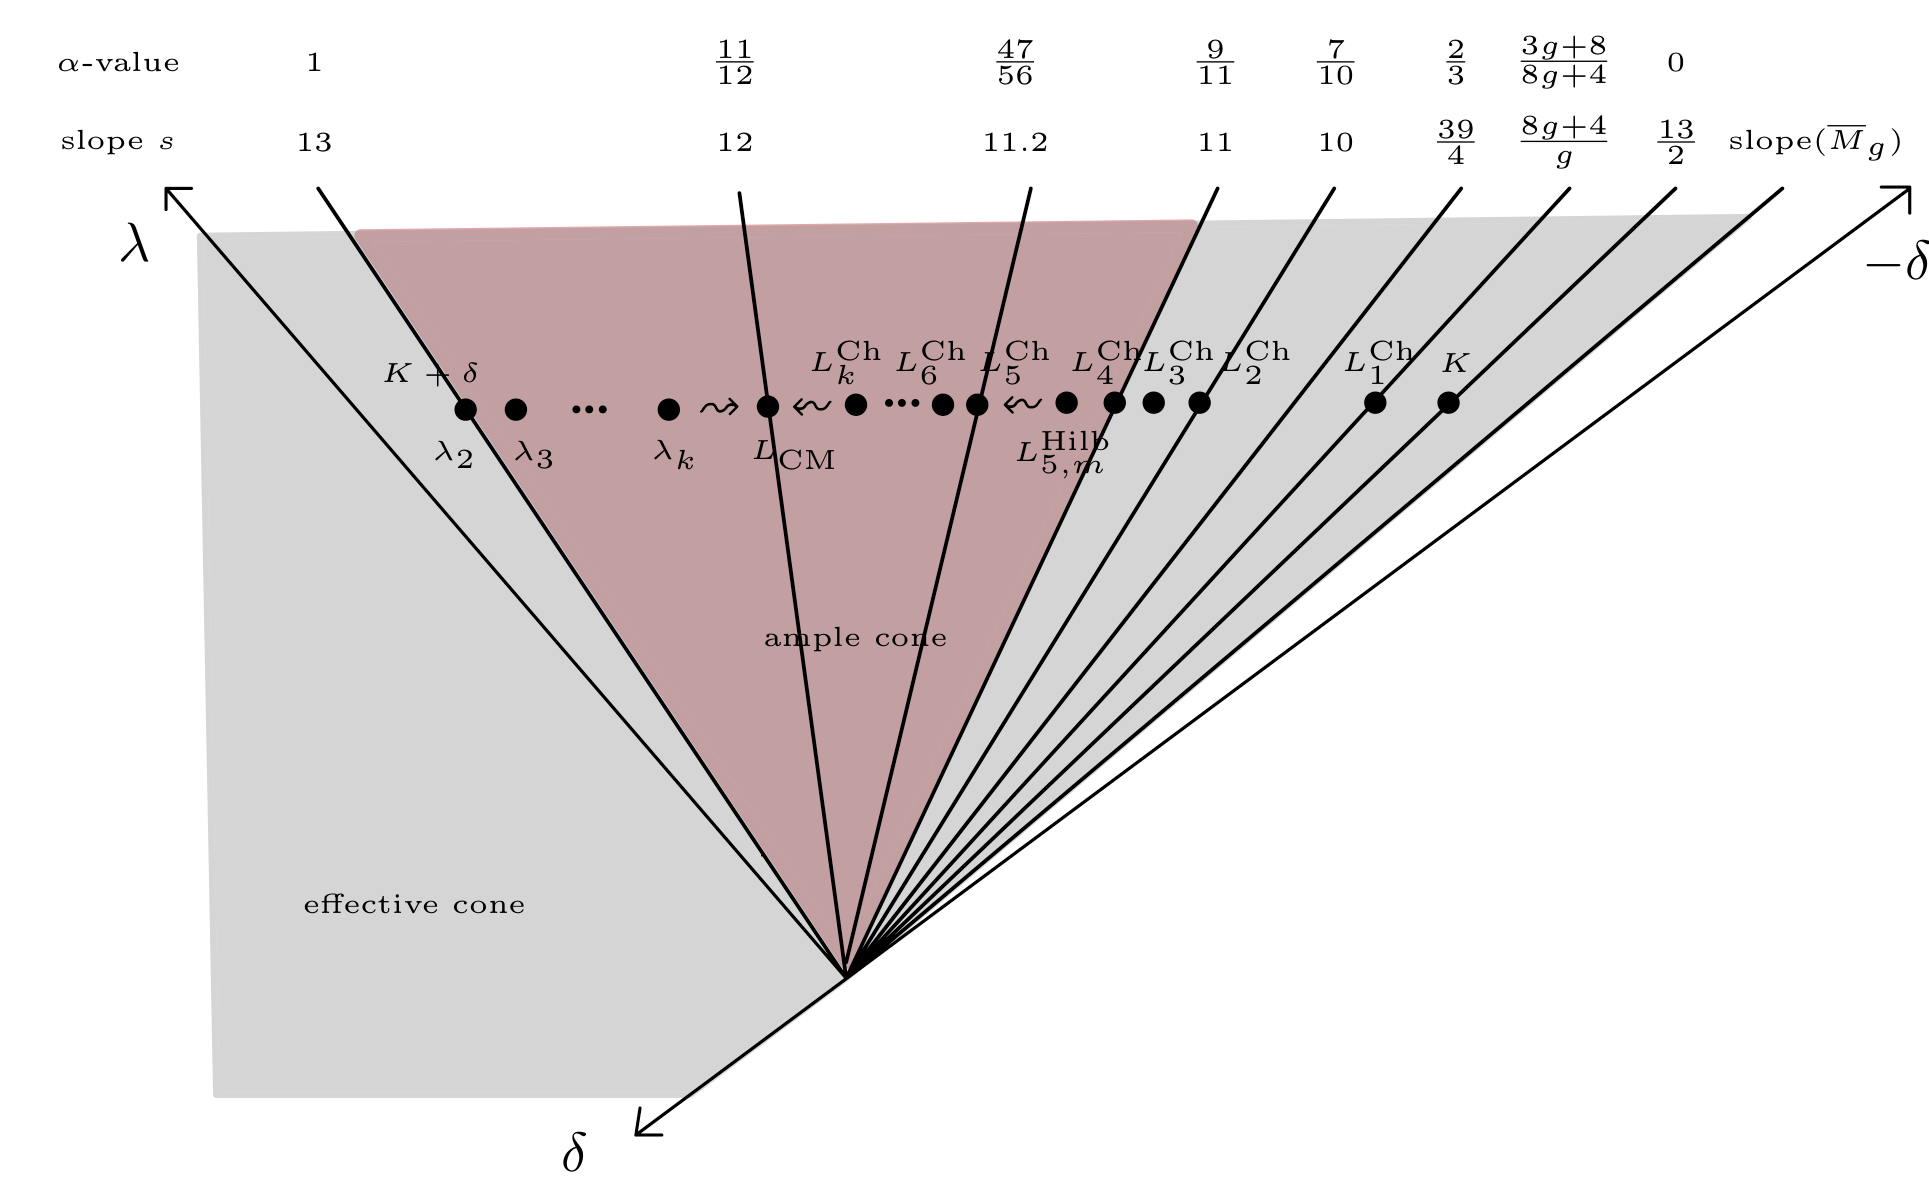
\includegraphics[width=.95\textwidth]{figures/moduli-cones.png}};
\begin{scope}[x={(im.south east)},y={(im.north west)}]
\fill[fill=white] (0.025937,0.964789) rectangle (0.096542,0.929577);
\node[font=\tiny,inner sep=0pt] at (0.061239,0.947183) {$\alpha$ 值};
\fill[fill=white] (0.027378,0.899061) rectangle (0.095101,0.862441);
\node[font=\tiny,inner sep=0pt] at (0.061239,0.880751) {斜率 $s$};
\fill[fill=white] (0.893372,0.899061) rectangle (0.991354,0.859155);
\node[font=\tiny,inner sep=0pt] at (0.942363,0.879108) {斜率 $(\overline M_g)$};
\fill[fill={rgb,255:red,213;green,213;blue,213}] (0.154179,0.252113) rectangle (0.275216,0.219249);
\node[font=\tiny,inner sep=0pt] at (0.214697,0.235681) {有效锥};
\fill[fill={rgb,255:red,194;green,159;blue,161}] (0.392507,0.477934) rectangle (0.494236,0.444601);
\node[font=\tiny,inner sep=0pt] at (0.443372,0.461268) {丰沛锥};
\end{scope}\end{tikzpicture}

\caption{$\lambda\delta$ 平面中的有效锥与丰沛锥}\label{src:6.10.12}
\end{figure}
\noindent\textbf{丰沛锥.} Kollár 判据 (\bookref{6.9.2}) 不仅给出 $\overline M_g$ 射影, 还给出当 $k\geq6$ 时 $\lambda_k$ 丰沛 (见注记~\bookref{6.9.4}). 线丛 $\lambda$ 数值有效; 它定义 Torelli 态射 $\overline M_g\to\overline A_g$. 因而当 $s>12$ 时 $s\lambda-\delta$ 丰沛. 注意关系式~\bookeqref{6.10.10} 蕴含 $L_{\mathrm{CM}}\sim\lim_{k\to\infty}\lambda_k$.

另一方面, GIT 构造对 $k\geq5$, $m\gg0$ 给出丰沛线丛 $L_k^{\mathrm{Ch}}$, $L_{k,\allowbreak m}^{\mathrm{Hilb}}$. 对其他 $k,\allowbreak m$, GIT 构造与 $\overline M_g$ 双有理的射影簇. 这些线丛的类成比例于
\[
\begin{aligned}
L_k^{\mathrm{Ch}}&\sim\begin{cases}(8+\frac4g)\lambda-\delta&\text{若 }k=1,\\(12-\frac4k)\lambda-\delta&\text{若 }k>1,\end{cases}\\
L_{k,m}^{\mathrm{Hilb}}&\sim\begin{cases}
\left(\dfrac{2+(m-1)((8g+4)m-2g+2))}{gm}\right)\lambda-\delta&\text{若 }k=1,\\
\left(\dfrac{12mk^2-4mk-4k+2}{mk^2}\right)\lambda-\delta&\text{若 }k>1;
\end{cases}
\end{aligned}
\]
见~\cite[定理 5.15]{Mum77}, \cite[第 2 节]{CH88} 与~\cite[第 1.5 节]{Vie89}. 固定 $k$, 有 $\lim_{m\to\infty}L_{k,\allowbreak m}^{\mathrm{Hilb}}\sim L_k^{\mathrm{Ch}}$, 而 $\lim_{k\to\infty}L_k^{\mathrm{Ch}}\sim L_{\mathrm{CM}}$. 取 $k=5$, 得到当 $s\geq11.2$ 时 $s\lambda-\delta$ 丰沛. 然而还可得到更强结论! Cornalba 与 Harris 从 GIT 推出的正性出发, 进一步证明 $s\lambda-\delta$ 丰沛当且仅当 $s>11$, 从而确定 $\operatorname{Pic}(\overline M_g)$ 的 $\lambda\delta$ 平面中的丰沛锥~\cite{CH88}. 完整的丰沛锥尚未确定, 但有一个有趣的 $F$-猜想: 它给出有限多个检验曲线, 并断言线丛丰沛当且仅当它与每条检验曲线的交数均为正. 这里不列举这些曲线, 但其中包括 $\overline{\mathcal M}_g$ 中参数化椭圆尾的有理曲线: 固定亏格 $g-1$ 的单标记曲线 $(C,\allowbreak p)$, 改变以结点方式附着的椭圆曲线 $(E,\allowbreak p)$ 的 $j$-不变量.

\noindent\textbf{有效锥与 Kodaira 维数.} 虽然 $\delta$ 显然是有效除子, 但使 $s\lambda-\delta$ 有效的最小 $s$, 即 $\overline M_g$ 的斜率, 并不清楚. 将 $g+1$ 写为 $(r+1)(s+1)$ 且 $s\geq3$, Harris 与 Mumford 定义 Brill--Noether 除子
\[
D_{\mathrm{BN}}:=\overline{\{[C]\mid C\text{ 具有一个 }g_d^r\}}\subseteq\overline{\mathcal M}_g,
\]
其类成比例于 $(g+3)\lambda-\frac{g+1}{6}\delta_0-\sum_{i=1}^{\lfloor g/2\rfloor}i(g-i)\delta_i$, 与 $r,\allowbreak s$ 无关; 见~\cite{HM82} 与~\cite[第 6.F 节]{HM98}. 当 $g$ 为奇数时, $D_{\mathrm{BN}}$ 的斜率为 $6+12/(g+1)$. 当 $g\geq24$ 时, 此斜率小于 $13/2$. 因 $K_{\overline{\mathcal M}_g}=13\lambda-2\delta$, 可推出 $K_{\overline{\mathcal M}_g}$ 位于有效锥的内部, 即下降为 $\overline M_g$ 上的大线丛. Eisenbud 与 Harris 将此推广到所有 $g\geq24$~\cite{EH87}. 因而对 $g\geq24$, $\overline M_g$ 的 Kodaira 维数为 $3g-3$, 且 $\overline M_g$ 为一般型.

这否定了 Severi 关于所有 $g$ 的 $\overline M_g$ 均为单有理的猜想. Severi 曾证明当 $g\leq10$ 时 $\overline M_g$ 单有理 (见~\bookref{1.1.2-subsection} 节), 现在已知对 $g\leq14$ 也成立~\cite{Ver05}. 对 $15$ 至 $23$ 之间的某些亏格, $\overline M_g$ 的 Kodaira 维数仍未知. 一般的 $\overline M_g$ 的斜率也未知. Harris 与 Mumford 曾猜想斜率至少为 $6+12/(g+1)$, 但 Farkas 与 Popa~\cite{FP05} 否定了它. 如今似乎存在不同看法: 有人认为 $\overline M_g$ 的斜率至多为 $6$, 也有人认为它趋于 $0$.

\noindent\textbf{$\overline M_g$ 的双有理几何.} Mumford 在利用 Chow 概形的 GIT 构造 $\overline M_g$ 的同一篇论文~\cite{Mum77} 中观察到, 其他 GIT 设置会给出 $\overline M_g$ 的双有理模型, 参数化奇点可能比结点更差的曲线. 具体地, 在亏格 $3$ 时, 他构造了有理映射
\[
\overline M_3\dashrightarrow\mathbb P(\operatorname{Sym}^4(\mathbb C^3))\mathbin{/\!/}\operatorname{SL}_3,
\]
将具有椭圆尾 (即通过结点附着的亏格 $1$ 曲线) 的曲线收缩为尖点曲线, 将椭圆桥 (即两条亏格 $1$ 曲线沿两点的结点并) 映为挠结点曲线, 并将超椭圆轨迹收缩为一点, 此点对应二重二次曲线.

因 $g\gg0$ 时 $\overline M_g$ 为一般型, 自然会问它的典范模型
\[
\overline M_g^{\mathrm{can}}=\operatorname{Proj}\bigoplus_d\Gamma(\overline{\mathcal M}_g,K_{\overline{\mathcal M}_g}^{\otimes d})
\]
是什么; 由~\cite{BCHM10}, 它是射影簇. $\overline M_g$ 是特别有趣的高维簇, 而其模描述为几何研究提供了切入点, 因而很适合用来检验极小模型纲领的工具. 为回答此问题, Hassett 在~\cite{Has05} 中提出考虑对数典范模型
\begin{equation}\label{src:6.10.13}
\overline M_g(\alpha):=\operatorname{Proj}\bigoplus_{d\geq0}\mathrm H^0(\overline{\mathcal M}_g,\lfloor d(K_{\overline{\mathcal M}_g}+\alpha\delta)\rfloor),
\end{equation}
从 $\overline M_g$ 过渡到 $\overline M_g^{\mathrm{can}}$, 其中 $\delta$ 为边界除子. 注意 $\overline M_g=\overline M_g(1)$ (因 $K+\delta$ 在 $\overline M_g$ 上丰沛), 而 $\overline M_g^{\mathrm{can}}=\overline M_g(0)$. 对任意亏格, Hassett 与 Hyeon 构造首个除子收缩 $\overline M_g\to\overline M_g(9/11)$~\cite{HH09}, 以及首个翻转
\[
\overline M_g(9/11)\longrightarrow\overline M_g(7/10)\longleftarrow\overline M_g(7/10-\epsilon),\qquad\epsilon\ll1
\]
~\cite{HH13}. 引人注目的是, 他们为每个射影簇给出模描述, 并证明首个收缩以尖点奇点替代椭圆尾, 首个翻转以挠结点曲线替代椭圆桥的轨迹.

存在参数化任意维数一般型簇的射影模空间, 因而很自然会把 $\overline M_g$ 看作这种模空间中的一点. Hacking 证明 $\overline{\mathcal M}_g$ 刚性, 即没有非平凡形变, 等价地 $\mathrm H^1(\overline{\mathcal M}_g,\allowbreak T_{\overline{\mathcal M}_g})=0$~\cite{Hac08}. 这印证了 Kapranov 的预期: 若 $X$ 为 $n$ 维光滑簇, 则迭代考虑参数化 $X$ 的形变的模空间 $X[1]$, 参数化 $X[1]$ 的形变的模空间 $X[2]$, 等等, 此过程恰在 $n$ 步后终止.

\noindent\textbf{$\overline M_g$ 的奇点.} 因 $\overline{\mathcal M}_g$ 光滑, 粗模空间的局部结构 (\bookref{5.4.13}) 推出 $\overline M_g$ 具有有限商奇点. Harris 与 Mumford 借助 Reid--Tai 判据证明 $\overline M_g$ 具有典范奇点~\cite{HM82}; 换言之, 多重典范截面延拓到 $\overline M_g$ 的奇点解消上. 这是他们证明 $\overline M_g$ 为一般型所必需的性质.

一般的亏格 $g\geq3$ 光滑曲线 $C\in\mathcal M_g(k)$ 具有平凡自同构群. 因 $\mathcal M_g$ 不可约, 只需给出一条自同构群平凡的光滑曲线便可推出此结论. 它意味着存在开子集 $U\subseteq\mathcal M_g$, 为光滑拟射影簇. 若 $g\geq4$, 非平凡自同构曲线的轨迹余维至少为 $2$, 且曲线 $[C]\in M_g$ 为奇点当且仅当 $\operatorname{Aut}(C)\ne1$. 见~\cite{Rau62,Pop69}.
